\documentclass[12pt]{scrartcl}
\usepackage[ngerman]{babel}


\usepackage{amsmath, amssymb}

\usepackage{array}  % for the tables

\usepackage{nameref}  % for referencing with name

\usepackage{hyperref}  % for hyperlinks

\usepackage{mathrsfs}

\usepackage{graphicx}  % for the images

\usepackage{xcolor, colortbl}

\usepackage{gensymb} % for \degree

\usepackage{pgfplots}

\usepackage{tabto}

\usetikzlibrary{arrows}

% \usepgfplotslibrary{external}

% \tikzexternalize

\definecolor{Gray}{gray}{0.85}

\setlength{\parindent}{0cm}

% hyperlinks
\hypersetup{
    colorlinks,
    citecolor=black,
    filecolor=black,
    linkcolor=black,
    urlcolor=black
}

\bibliographystyle{IEEetran}




\author{David Jäggli}

\title{Diskrete Mathematik}



% ---------- Begin Main Document ----------- %



\begin{document}

\maketitle

\tableofcontents

\newpage
\section{Allg}

\subsection{Grundlagen der Logik und Beweise}

\begin{itemize}
    \item Die Regeln der Logik geben mathematischen Aussagen eine präzise Bedeutung.
    \item Konstruktion korrekter mathematischer Argumente
\end{itemize}

\subsection{Aussagen (Propositionen)}
\textbf{Propositionen:}
\begin{itemize}
    \item Bern ist die Bundesstadt
    \item 1 + 1 = 2
    \item Goldbachsche Vermutung: sie ist entweder wahr oder falsch, man weis es noch nicht
\end{itemize}

\textbf{Keine Propositionen:}
\begin{itemize}
    \item Wie spät ist es?
    \item x + 1 = 2
    \item Dieser Satz ist falsch.
\end{itemize}

Begründung: Es handelt sich hier nicht um Aussagen, die entweder wahr oder falsch sind.
Eine Aussage ist wahrheitsdefiniert. In einer Aussage darf nicht offen sein ob die Aussage wahr oder 
falsch sein kann. Sie darf sich auch nicht selbst widersprechen.

% ------------------------------------------------------
\section{Operatoren}

\begin{itemize}
    \item Negotiationsoperator: $\lnot$
    \item Konjunktion $\land$
    \item Disjunktion $\lor$
    \item Implikation $\rightarrow$
    \item Bikonditional $\leftrightarrow$
\end{itemize}



\subsection{Diskunktion}
$p \lor q$\\
Wenn p oder q wahr ist, ist die Aussage wahr (logic OR).


\renewcommand{\arraystretch}{1.5}
\begin{tabular}{ | m{3em} | m{3em} | m{3em} | }
    \hline
    p & q & $p \lor q$\\ 
    \hline
    w & w & w\\ 
    \hline
    w & f & w\\ 
    \hline
    f & w & w\\ 
    \hline
    f & f & f\\ 
    \hline
\end{tabular}


\subsection{Implikation}
$p \rightarrow q$\\
Wenn p dann q


\renewcommand{\arraystretch}{1.5}
\begin{tabular}{ | m{3em} | m{3em} | m{3em} | }
    \hline
    p & q & $p \rightarrow q$\\ 
    \hline
    w & w & w\\ 
    \hline
    w & f & f\\ 
    \hline
    f & w & w\\ 
    \hline
    f & f & w\\ 
    \hline
\end{tabular}


\subsection{Bikonditional}
$p \leftrightarrow q$\\
Wenn beide den gleichen Wahrheitswert haben ist die Aussage wahr.\\
\textbf{Wahrheitstabelle:}\\

\renewcommand{\arraystretch}{1.5}
\begin{tabular}{ | m{3em} | m{3em} | m{3em} | }
    \hline
    p & q & \(p \leftrightarrow q\)\\ 
    \hline
    w & w & w\\ 
    \hline
    w & f & f\\ 
    \hline
    f & w & f\\ 
    \hline
    f & f & w\\ 
    \hline
\end{tabular}

\subsection{Prioritäten}
\renewcommand{\arraystretch}{1.5}
\begin{tabular}{ | m{4em} | m{4em} | }
    \hline
    Operator & Priorität\\ 
    \hline
    $\lnot$ & 1\\ 
    \hline
    $\land$ & 2\\ 
    \hline
    $\lor$ & 2\\ 
    \hline
    $\rightarrow$ & 3\\ 
    \hline
    $\leftrightarrow$ & 3\\ 
    \hline
\end{tabular}


\section{Aussagen}

\subsection{Tautologie und Wiederspruch}
Tautologie ist eine Aussage, welche immer wahr ist.\\
Ein Wiederspruch ist eine Aussage, welche immer falsch ist.

\subsection{Logische Äquivalenzen}
Die Aussage p und q heissen logisch äquivalent, falls \(p \leftrightarrow q\) eine Tautologie ist. 
Man schreibt dann \(p \Leftrightarrow q\) oder
\(p \equiv q\) bzw. $p \sim q$

\subsection{Logische Äquivalenzregeln}
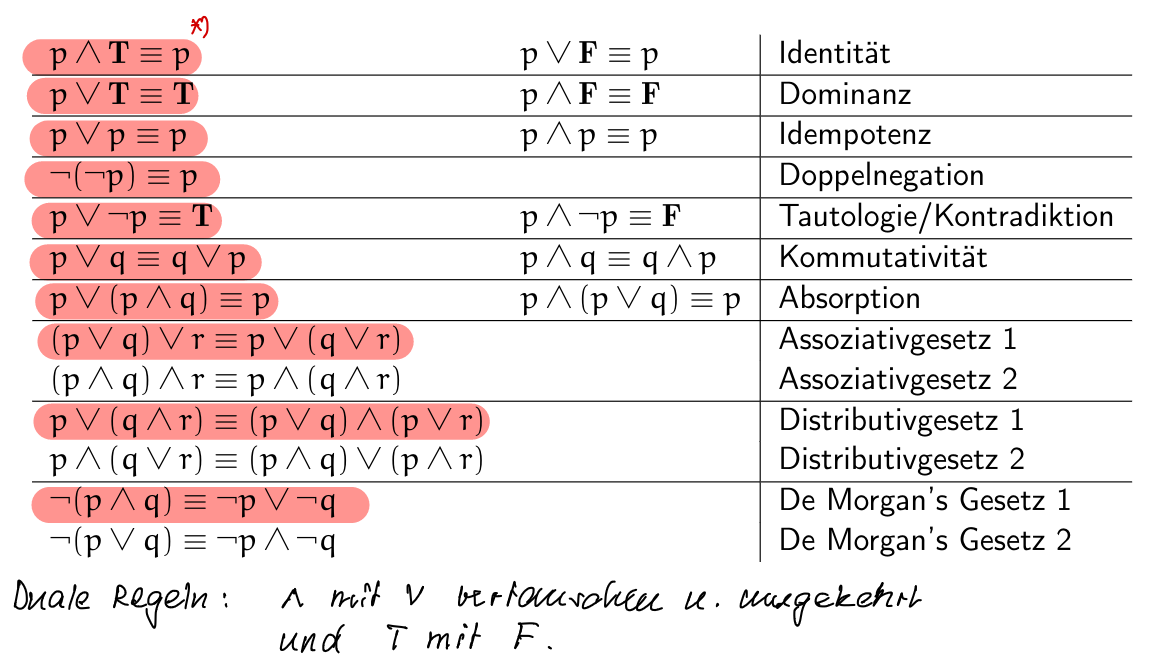
\includegraphics[width=14cm]{img/logic_equivalence_rules.png}

\newpage
\textbf{Beispiel angewandte logische Äquivalenzregeln}\\
Beispiel 1:\\
$\left(p \lor \lnot(q \land p)\right) \land \left(r \lor (s \lor r)\right)$\\
$\equiv (p \lor \lnot q \lor \lnot p) \land (r \lor r \lor s)$\\
$\equiv (T \lor \lnot q) \land (r \lor s)$\\
$\equiv T \land (r \lor s)$\\
$\equiv r \lor s$
 \\
 \\
 \\

Beispiel 2:\\
$(a \rightarrow (b \rightarrow c)) \rightarrow ((a \rightarrow b)\rightarrow (a \rightarrow c))$\\
$\equiv (a \rightarrow (\lnot b \lor c)) \rightarrow ((\lnot a \lor b) \rightarrow (\lnot a \lor c))$\\
$\equiv (\lnot a \lor (\lnot b \lor c)) \rightarrow (\lnot(\lnot a \lor b) \lor (\lnot a \lor c))$\\
$\equiv (\lnot a \lor \lnot b \lor c) \rightarrow ((a \land \lnot b) \lor \lnot a \lor c)$\\
$\equiv (\lnot a \lor \lnot b \lor c) \rightarrow ((a \lor \lnot a) \land (\lnot b \lor \lnot a) \lor c)$\\
$\equiv (\lnot a \lor \lnot b \lor c) \rightarrow (\lnot b \lor \lnot a \lor c)$\\
$\equiv$ X $\rightarrow$ X\\
$\equiv \lnot$X $\lor$ X\\
$\equiv$ T\\

\section{Quantoren}
Wird ein Quantor auf die Variable x angewandt, dann nennt man diese Variable \textit{gebunden}, ansonsten \textit{frei}.
\subsection{Prädikate}
Ein Prädikat ist ein Wortkonstrukt, welches mindestens eine Variable enthält.\\
$P(x) =$ ''$x > 3$''\\
Die Aussage $P(4) = 4 > 3$ ist wahr, während $P(2) = 2 > 3$ falsch ist.

\subsection{Allquantor}
Ist $P(x)$ wahr für alle x aus einer bestimmten Universalmenge, dann schreibt man $\forall x P(x)$.
Gelesen wird dies, "für alle $x$ gilt $P(x)$".\\
Falls es nur auf eine Bestimmte Zahlenmenge zutrifft (z.B. $\mathbb{Z}$) dann schreibt man:\\
$\forall x \in \mathbb{Z}$ ist wahr.

\subsection{Existenzquantor}
Ist $P(x)$ wahr für mindestens ein $x$ aus einer bestimmten Universalmenge, dann schreibt man $\exists x P(x)$
und liest: "es existiert ein $x$ für welches $P(x)$ wahr ist".


\subsection{Verschachtelte Quantoren}
Die Reihenfolge der Quantoren ist wesentlich; ausser alle Quantoren sind vom gleichen Typ (also Allquantoren oder Existenzquantoren)!


\newpage
\section{Beweise}
\begin{itemize}
    \item Ein Satz (Theorem) ist eine Aussage, von der man zeigen kann, dass sie wahr ist.
    \item Um zu zeigen, dass ein Satz wahr ist, verwendet man eine Abfolge (Sequenz) von Aussagen, die zusammen ein Argument, genannt Beweis ergeben.
    \item Aussagen können Axiome oder Postulate enthalten (grundlegende Annahmen der mathematischen Strukturen).
    \item Durch logisches (also gewissn Regeln gehorchendes) Schliessen werden Folgerungen gemacht, die zusammen den Beweis ergeben.
    \item Ein Lemma ist ein einfacher Satz, der in Beweisen von komplizierteren Sätzen verwendet wird.
    \item Ein Korollar ist eine einfache Folgerung eines Satzes.
\end{itemize}


$5 \times 3 \cdot 12 = 27$



% tabular example 3 columns
% \renewcommand{\arraystretch}{1.5}
% \begin{center}
%     \begin{tabular}{ | m{12em} | m{12em} | m{12em} | }
%         \hline
%         1 & 2 & 3\\ 
%         \hline
%         1 & 2 & 3\\ 
%         \hline
%         1 & 2 & 3\\ 
%         \hline
%     \end{tabular}
% \end{center}


% tabular example 2 columns
% \renewcommand{\arraystretch}{1.5}
% \begin{center}
%     \begin{tabular}{ | m{17em} | m{17em} | }
%         \hline
%         1 & 2\\ 
%         \hline
%         1 & 2\\ 
%         \hline
%         1 & 2\\ 
%         \hline
%     \end{tabular}
% \end{center}


% \begin{tikzpicture}[line cap=round,line join=round,>=triangle 45,x=0.5cm,y=0.25cm]
%     \begin{axis}[
%     x=0.75cm,y=0.5cm, % size of the grid
%     axis lines=middle,
%     ymajorgrids=true,
%     xmajorgrids=true,
%     xmin=-10,
%     xmax=10,
%     ymin=-10,
%     ymax=10,
%     xtick={-11,-10,...,10},
%     ytick={-10,-9,...,9},]
%     \draw[line width=2pt,color=blue] (-10,-5) -- (-2,-1);
%     \begin{scriptsize}
%         \draw[color=blue] (-9.866,-4.728) node {$g$};
%         \draw[color=blue] (-1.906,7.172) node {$f$};
%         \draw[color=blue] (3.134,5.232) node {$h$};
%     \end{scriptsize}
% \end{axis}
% \end{tikzpicture}




% \bibliography{quantum_ready}

\end{document}